\documentclass[12pt]{article}
\usepackage[margin=1in]{geometry}
\usepackage[x11names]{xcolor}
\usepackage{float}  
\usepackage{amsmath}
\usepackage{amssymb}
\usepackage{graphicx}
\usepackage{hyperref}
\usepackage{mdframed}
\usepackage{listings}

\lstset{
  basicstyle=\ttfamily,
  frame=single,
  numbers=left,
  numberstyle=\tiny,
  stepnumber=1,
  breaklines=true
}
\hypersetup{
    colorlinks=true,
    linkcolor=black,
    citecolor=blue,
    filecolor=blue,
    urlcolor=gray
}
\newmdenv[
  backgroundcolor=gray!10,
  linecolor=black,
  innerleftmargin=10pt,
  innerrightmargin=10pt,
  innertopmargin=10pt,
  innerbottommargin=10pt,
  roundcorner=5pt,
  linewidth=1pt,   
]{definitionbox}

\title{\textbf{Distributed Bitonic Sort with MPI}}
\author{Maria Charisi\\Maria Kostomanolaki}
\date{\today}

\begin{document}

\maketitle

\tableofcontents

\vfill
\begin{center}
    \textit{Professor: Nikolaos Pitsianis\\
    Department of Electrical and Computer Engineering\\
    Parallel and Distributed Systems}
\end{center}
\newpage

\section{Serial Bitonic Sort}

Understanding \textit{Distributed Bitonic Sort} requires first examining the serial implementation of the algorithm.

\subsection{Bitonic Sequence}

\begin{definitionbox}
A \textbf{Bitonic Sequence} is a sequence of integers that first increases monotonically and then decreases monotonically (or vice versa). The reverse of a bitonic sequence or any cyclic rotation of it also forms a bitonic sequence.
\end{definitionbox}

For example, the sequence [6, 4, 3, 1, 2, 5, 8, 7] is bitonic, because when the last 7 is rotated to the beginning, the resulting sequence is decreasing and then increasing.


\subsection{Bitonic Merge}

\begin{definitionbox}
\textbf{Bitonic Theorem:} The element-wise comparison of the first half of a bitonic sequence with its second half, along with the separation into minima and maxima subsequences, also results in bitonic sequences.
\end{definitionbox}

\textbf{Bitonic Merge} is a function that takes a bitonic sequence as input, where the length is a power of two, and outputs a sorted sequence. Bitonic Merge recursively applies the \textit{Bitonic Theorem} and stores first the minima and then the maxima sequence, as demonstrated in the following example:

\begin{figure}[H]
    \centering
    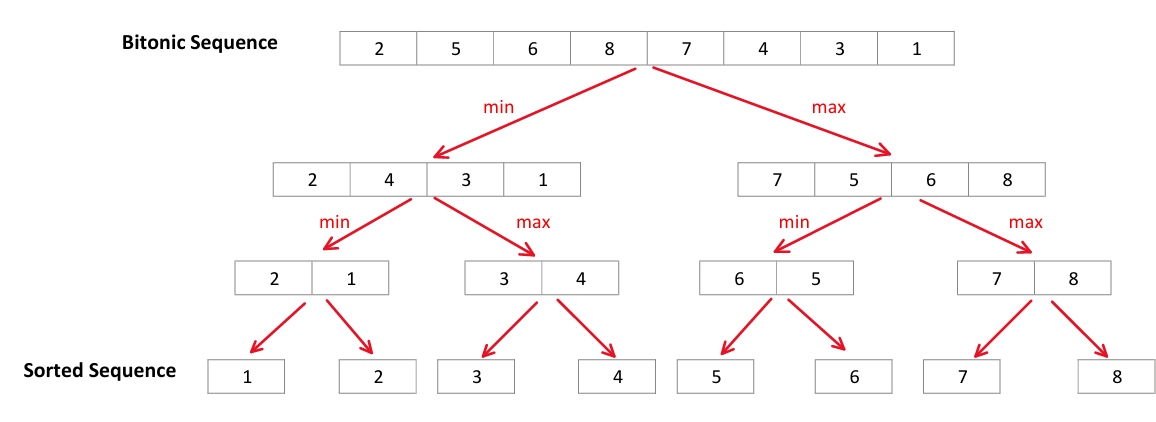
\includegraphics[width=0.9\linewidth]{serialBitonic.png}
    \caption{Bitonic Merge}
    \label{fig:enter-label}
\end{figure}

If we assume that the input sequence has length $n$, then:

\begin{itemize} 
\item Element-wise comparisons between the two halves of the sequence have a time complexity of $O(n)$.
\item Bitonic Merge calls itself twice: once for the minima sequence and once for the maxima sequence. Therefore, it is recursively called $log(n)$ times. 
\end{itemize}

\begin{lstlisting}[language=C]
    for(int i = 0; i < m; i++){
        if(arr[i] > arr[i+m]){
            min.arr[i] = arr[i+m];
            max.arr[i] = arr[i];
        } 
        else {
            min.arr[i] = arr[i];
            max.arr[i] = arr[i+m];
        }
    }

    min = bmerge(min, order);
    max = bmerge(max, order);
\end{lstlisting}
\vspace{0.3cm}
So, the \textbf{time complexity} of Bitonic Merge is:
\[T_M(n) = 2T_M(n/2) + O(n) = O(nlog(n))\]

\subsection{Bitonic Sort}
\textit{Bitonic Sort} takes an arbitrary sequence of integers as input and transforms it into a bitonic sequence. It achieves this by recursively calling itself, sorting the first half in one direction and the second half in the opposite direction. The next step is to call \textit{Bitonic Merge} to sort the resulting bitonic sequence.
\vspace{0.3cm}
\begin{lstlisting}[language=C]
    l = bsort(l, true); //First half ascending order
    r = bsort(r, false); //Second half descending order

    // Create the bitonic sequence
    for(int i = 0; i < m; i++){
        b.arr[i] = l.arr[i];
        b.arr[i + m] = r.arr[i];
    }

    b = bmerge(b, order);
\end{lstlisting}
\vspace{0.3cm}
Taking into account the algorithm above, the \textbf{time complexity} of the Bitonic Sort is:

\[T_S(n) = 2 T_S(n/2) + T_M(n) = O(n (\log n)^2)\]

\newpage

\section{Distributed Bitonic Sort}

We can understand that there are serial sorting algorithms that have much better performance than the bitonic sort. Specifically, bitonic sort has \(O(n (\log n)^2)\) complexity, whereas other algorithms such as merge sort have \(O(n \log n)\) complexity. However, bitonic sort is useful because it is well-suited for parallel and distributed implementations.

The \textit{Distributed Bitonic Sort} takes two integers, \( p \) and \( q \), as input. \( p \) defines the number of processes, specifically \textbf{\( 2^p \) processes} will start, and each process will handle \textbf{\( 2^q \) numbers}. In the end, every process will sort its numbers locally. If we then gather all the numbers from all processes in order (first the chunk from the first process, and so on), we will end up with a sorted sequence in ascending order. The final sequence will have a length of \( N = 2^{p+q} \). Inner-process communication will be achieved by using \textbf{Message Passing Interface (MPI)}.

\subsection{Brief Explanation}
As an introduction, we will briefly analyze the algorithm step by step. As we already mentioned, we start with \(2^p\) processes, and every process takes a sequence of length \(2^q\).

\begin{itemize}
    \item At first, every process will sort its sequence in ascending or descending order (based on the rank of the process). For this sorting, we will use the \texttt{qsort()} function from the C \texttt{stdlib} library, with complexity \(O(n \log n)\).
    
    \item Next, we will enter a loop that will execute \(p\) times. At every iteration (stage), processes will communicate and exchange elements. Specifically, in the first iteration, there will be one step of communication, in the second, two steps, and so on.
    
    \item These communications will not be random. At each step, each process will communicate with a specific partner at a certain distance. They will compare their numbers elementwise, and depending on the current stage, one will keep the minimums, and the other will keep the maximums.
    
    \item At the end of each iteration, each process will end up with a bitonic sequence, which will be sorted again using the \texttt{elbowsort} function instead of \texttt{qsort}. The \texttt{elbowsort} function has \(O(n)\) complexity and only sorts bitonic sequences.
\end{itemize}

\begin{lstlisting}[language=C]
    firstSort(local, ascdesc(rank, 0));

    for (int stage = 1; stage <= log2(size); stage++){
        for (int step = stage; step > 0; step--){
            int distance = 1 << (step - 1);
            int partner_rank = partner(rank, distance);
            Sequence remote = exchange(partner_rank, local);
            minmax(rank, stage, distance, local, remote);
            deleteSeq(remote);
        }
        elbowSort(local, ascdesc(rank, stage));
    }
\end{lstlisting}

The functions \texttt{partner}, \texttt{exchange}, \texttt{minmax}, \texttt{ascdesc}, and \texttt{elbowSort} will be explained further.

\begin{figure}[H]
    \centering
    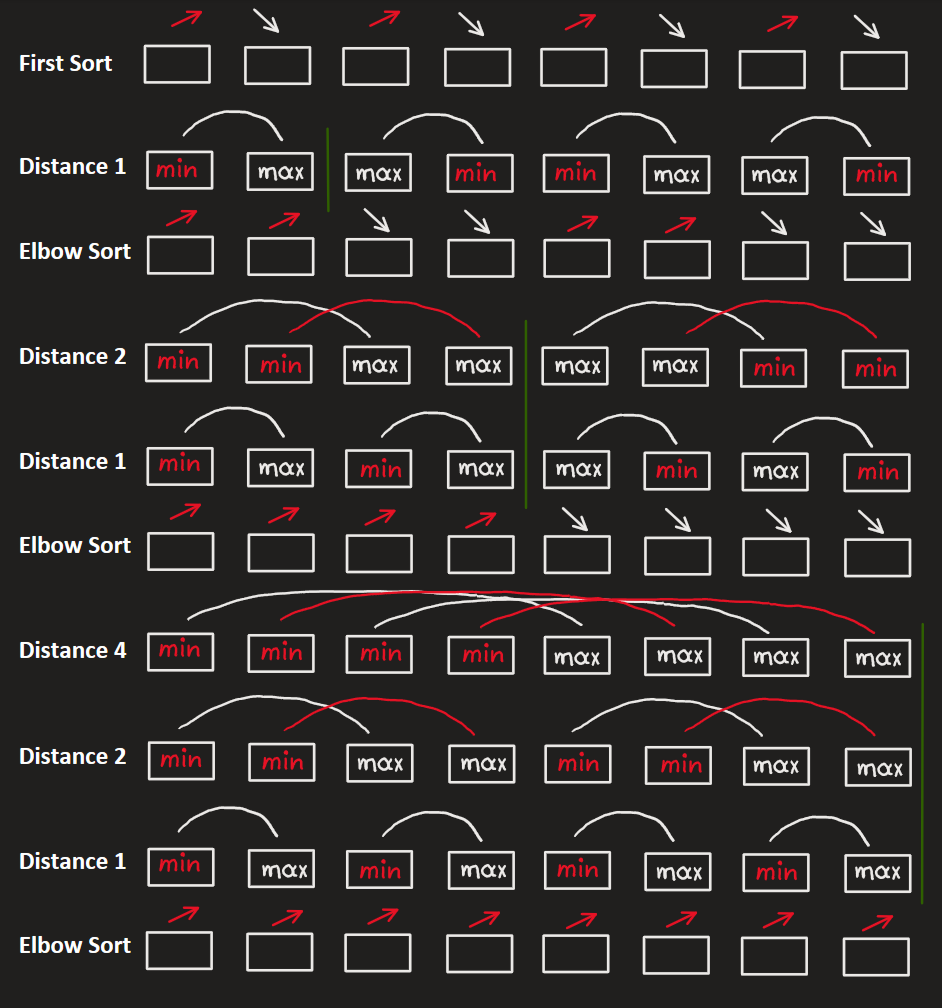
\includegraphics[width=0.9\linewidth]{distributedBitonic.png}
    \caption{Distributed Bitonic for 8 processes}
    \label{fig:enter-label}
\end{figure}

In the above figure, the rectangle represents a process. Each row is a step of the algorithm, and it is either a communication step or a sorting step.
\newpage

\subsection{Partner}
The rank of the partner process can be easily calculated if the current communication distance is known. The distance depends on the current stage of the algorithm, is always a power of two, and ranges from \( 2^{\text{stage}-1} \text{ to } 2^0 \)

\[\text{rank} \oplus \text{distance}\]
\begin{table}[h]
    \centering
    \begin{tabular}{|c|c|c|c|c|}
        \hline
        \textbf{Decimal} & \textbf{Binary} & \textbf{XOR with 1} & \textbf{XOR with 2} & \textbf{XOR with 4} \\ \hline
        0 & 000 & 001 & 010 & 100 \\ \hline
        1 & 001 & 000 & 011 & 101 \\ \hline
        2 & 010 & 011 & 000 & 110 \\ \hline
        3 & 011 & 010 & 001 & 111 \\ \hline
        4 & 100 & 101 & 110 & 000 \\ \hline
        5 & 101 & 100 & 111 & 001 \\ \hline
        6 & 110 & 111 & 100 & 010 \\ \hline
        7 & 111 & 110 & 101 & 011 \\ \hline
    \end{tabular}
    \caption{XOR Table}
    \label{tab:xor}
\end{table}

\subsection{Exchange Data}
Communication between processes is achieved through the \texttt{exchange} function. Each process uses \texttt{MPI\_Sendrecv} to send its local data to its partner and store the received data from the partner in a buffer called \texttt{remote}.
\vspace{0.3cm}
\begin{lstlisting}[language=C]
    Sequence exchange(int partner, Sequence local)
    {
        Sequence remote = createSeq(local.size);
        MPI_Sendrecv(local.arr, local.size, MPI_INT, partner, 0, remote.arr, remote.size, MPI_INT, partner, 0, MPI_COMM_WORLD, MPI_STATUS_IGNORE);
        return remote;
    }
\end{lstlisting}

\subsection{Maxima or Minima}
Each process compares all its local elements with the remote ones element-wise and keeps either the \textbf{minimums} or the \textbf{maximums}. This decision is crucial for the final result and depends on the current stage and distance.

To understand the motif behind the algorithm, we can imagine that at each stage, a mirror is placed before the process with rank \( 2^{\text{stage}} \). These mirrors are depicted in Figure 2 with green vertical lines. Each mirror has a width equal to \( 2 \times 2^{\text{stage}} \), and the processes with ranks in the range \([0, 2^{\text{stage}} - 1]\) are reflections of the processes with ranks in the range \([2^{\text{stage}}, 2 \times 2^{\text{stage}} - 1]\). This pattern repeats until the end of the sequence.

Taking advantage of this motif, we simply calculate the modulo of the rank with the width of the mirror and then find the reflection of the outcome from the first mirror. The ranks that are placed to the left and right of the mirror have a reflection equal to zero, and so on. 

Now that we have the reflection, the criterion that determines whether the process will keep the minimums or the maximums is the distance. Specifically, we will retain the \( \log_2(\text{distance}) \)-th bit from the right of the rank. If this bit is equal to zero, the process will keep the maximums; otherwise, it will keep the minimums.

\vspace{0.3cm}
\begin{lstlisting}[language=C]
void minmax(int rank, int stage, int distance, Sequence local, Sequence remote)
{
    int mirror = 1 << stage;
    int w = 2 * mirror;
    int pos = rank % w;

    int reflection = pos < mirror ? mirror - pos - 1 : pos - mirror;

    if (reflection & (1 << (int)log2(distance))){
        // Keep min elements (element-wise)
    }
    else{
        // Keep max elements (element-wise)
    }
}

\end{lstlisting}

\begin{table}[h]
    \centering
    \begin{tabular}{|c|c|c|c|c|}
        \hline
        \textbf{Decimal} & \textbf{Rank} & \textbf{Reflection} & \textbf{Distance 1} & \textbf{Distance 2} \\ \hline
        0 & 000 & 0\textcolor{blue}{1}\textcolor{blue}{1} & \textcolor{blue}{min} & \textcolor{blue}{min} \\ \hline
        1 & 001 & 0\textcolor{blue}{1}\textcolor{red}{0} & \textcolor{red}{max} & \textcolor{blue}{min} \\ \hline
        2 & 010 & 0\textcolor{red}{0}\textcolor{blue}{1} & \textcolor{blue}{min} & \textcolor{red}{max} \\ \hline
        3 & 011 & 0\textcolor{red}{0}\textcolor{red}{0} & \textcolor{red}{max} & \textcolor{red}{max} \\ \hline
        4 & 100 & 0\textcolor{red}{0}\textcolor{red}{0} & \textcolor{red}{max} & \textcolor{red}{max} \\ \hline
        5 & 101 & 0\textcolor{red}{0}\textcolor{blue}{1} & \textcolor{blue}{min} & \textcolor{red}{max} \\ \hline
        6 & 110 & 0\textcolor{blue}{1}\textcolor{red}{0} & \textcolor{red}{max} & \textcolor{blue}{min} \\ \hline
        7 & 111 & 0\textcolor{blue}{1}\textcolor{blue}{1} & \textcolor{blue}{min} & \textcolor{blue}{min} \\ \hline
    \end{tabular}
    \caption{Stage 2 for 8 processes}
    \label{tab:xor}
\end{table}
\newpage

\subsection{Ascending or Descending}
At the end of every stage, each process sorts its elements in ascending or descending order. The function \texttt{ascdesc} defines this order in a manner similar to the approach used previously with the reflection. For example, in the first sort (stage 0), we keep the first bit from the right. If this bit is equal to zero, the process sorts its local array in ascending order; otherwise, it sorts it in descending order.
\[\texttt{rank} \ \&  \ (1 \ll \texttt{stage})\]

\subsection{Elbow Sort}
As we have mentioned earlier, at the end of each stage, all processes will have a bitonic sequence. Therefore, instead of using \texttt{qsort} for sorting the sequence, we will use \texttt{elbowSort}.

The function \texttt{elbowSort} takes a bitonic sequence as input and sorts it in the desired order. It begins by identifying the \textbf{"elbow"} of the bitonic sequence. We define the elbow of a bitonic sequence as the element such that all elements before it are monotonically decreasing (or increasing), and all elements after it are monotonically increasing (or decreasing). 

It is clear that only the elements with the \textbf{minimum} or \textbf{maximum} value can serve as the elbow of the sequence. If these elements were placed elsewhere, they would disrupt the monotonic increase or decrease. Furthermore, sequences like \([6, 4, 3, 1, 2, 5, 8, 7]\) are not problematic because they always have a cyclic rotation with a correct elbow candidate, like this one \([7, 6, 4, 3, 1, 2, 5, 8]\).

In our case, we choose the minimum element as the elbow and take advantage of the fact that all the elements before and after it are already sorted. We place the elbow in the correct position (at the beginning if we are sorting in ascending order, or at the end if sorting in descending order). Then, we place \textbf{two pointers}: one to the \textbf{left} and one to the \textbf{right} of the elbow.
\vspace{0.3cm}
\begin{lstlisting}[language=C]
    int l = (elbowIndex - 1 + s.size) % s.size;
    int r = (elbowIndex + 1) % s.size;
\end{lstlisting}
\vspace{0.3cm}
From this point, we compare the two pointers. The smaller element will take the next position in the sequence. The pointer corresponding to the smaller element will then move one step to the right (if referring to the right pointer) or one step to the left (if referring to the left pointer). This process continues until the entire sequence is sorted.

When a pointer reaches the end of the sequence, it will wrap around to the beginning (and vice versa for the opposite pointer). This way, we ensure that cases like the one we mentioned earlier are sorted correctly.
\newpage

\vspace{0.3cm}
    \begin{lstlisting}[language=C]
    // Sorting in ascending order
    int sortedIndex = 0;
    sortedSeq.arr[sortedIndex++] = s.arr[elbowIndex];
    
    while (sortedIndex < s.size)
    {
        if (s.arr[l] < s.arr[r])
        {
            sortedSeq.arr[sortedIndex++] = s.arr[l];
            // Wrap around to end if l < 0
            l = (l - 1 + s.size) % s.size;
        }
        else
        {
            sortedSeq.arr[sortedIndex++] = s.arr[r];
            // Wrap around to start if r >= s.size
            r = (r + 1) % s.size;
        }
    }
\end{lstlisting}
\newpage
\section{Results}
For testing, we executed our program on the \textbf{Rome} partition of the \textbf{Aristotle cluster}, provided by Aristotle University of Thessaloniki. The Rome partition consists of 17 nodes with 128 CPU cores per node. To test our program, we utilized all 128 CPU cores of a single node, and the following results were obtained:

\begin{figure}[H]
    \centering
    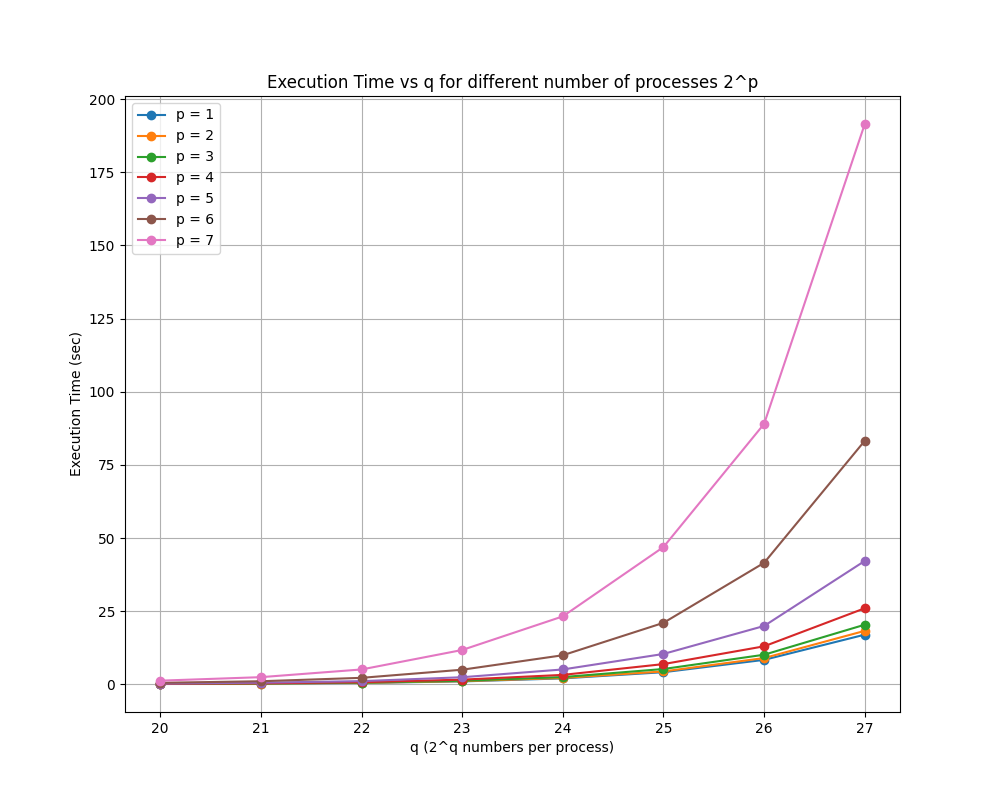
\includegraphics[width=0.9\linewidth]{results.png}
    \caption{Performance}
    \label{fig:enter-label}
\end{figure}

\end{document}
